\section{滤波器}

这一章主要讨论滤波器的设计和实现。滤波器是信号处理中的一个重要部分,
它可以用来去除噪声,提取信号,以及对信号进行分析。滤波器的设计是一个复杂的过程,
需要根据具体的应用来选择合适的滤波器类型和参数。
在本章中,我们将讨论滤波器的基本原理,以及如何设计和实现滤波器。

\begin{note}
    此小节还未完成。
\end{note}

\subsection{滤波器的表示}

\begin{definition}
    \bd{滤波器}是以特定方式改变信号的频率特性,从而变换信号的处理系统。
    滤波器一般有如下类别,如图 \ref{fig:filter_types} 所示:
    \begin{enumerate}[label=(\arabic*)]
        \item 高通滤波器(HP)
        \item 低通滤波器(LP)
        \item 带通滤波器(BP)
        \item 带阻滤波器(BS)
        \item 全通滤波器(AP)
    \end{enumerate}
    \begin{figure}[H]
        \centering
        \includegraphics[width=0.8\textwidth]{chap4/img/filter_types.png}
        \caption{滤波器类型}
        \label{fig:filter_types}
    \end{figure}

    滤波器也可以被分为\bd{模拟滤波器}和\bd{数字滤波器}。
    \begin{itemize}
        \item \bd{模拟滤波器}是由电阻、电容、电感等部件构成的电路。
            滤波器特性对所用部件的物理标称值非常敏感,而且,
            有些部件的物理特性会随温度变化而改变。
        \item \bd{数字滤波器}是用软件实现的,很少依赖硬件。滤波软件
            只是一系列程序指令。虽然它是在硬件平台上运行,但
            是硬件平台本身并不决定滤波器的性能。数字滤波器的
            性能是由\bd{一组系数}确定的。
    \end{itemize}
    数字滤波器的实现方式一般有以下几种:
    \begin{enumerate}
        \item 用流图计算滤波器的输出。
        \item 用差分方程计算滤波器的输出。
        \item 用卷积过程计算滤波器的输出。
        \item 用 DTFT 直接改变信号频谱。
    \end{enumerate}
\end{definition}

\begin{definition}
    模拟
\end{definition}

\begin{example}
    \label{exercise:serial-flow-chart}
    写出如图 \ref{fig:serial-flow-chart} 所示级联流图的差分方程。
    \begin{figure}[H]
        \centering
        \includegraphics[width=0.8\textwidth]{chap4/img/serial_flow_chart.png}
        \caption{例 \theexample~ 的级联流图}
        \label{fig:serial-flow-chart}
    \end{figure}
\end{example}

\begin{solution}
    不妨设 $x(n) = x_1(n), y(n) = y_3(n)$,
    以及 $y_1(n) = x_2(n), y_2(n) = x_3(n)$,则如图 \ref{fig:serial-flow-chart-annotated} 所示,
    \begin{align*}
        y_1(n) & = x_1(n) - 0.1x_1(n - 1) + 0.2x_1(n - 2), \\
        y_2(n) & = x_2(n) + 0.3x_2(n - 1) + 0.1x_2(n - 2), \\
        y_3(n) & = x_3(n) - 0.4x_3(n - 1).
    \end{align*}
    \begin{figure}[H]
        \centering
        \includegraphics[width=0.8\textwidth]{chap4/img/serial_flow_chart_annotated.png}
        \caption{例 \theexample~ 的级联流图(带标注)}
        \label{fig:serial-flow-chart-annotated}
    \end{figure}
    将 $y_1(n)$ 代入 $y_2(n)$ 的表达式中,将 $y_2(n)$ 代入 $y_3(n)$ 的表达式中,
    可得级联流图的差分方程为
    \begin{align*}
        y_3(n) = x_1(n) - 0.2x_1(n - 1) + 0.19x_1(n - 2) - 0.058x_1(n - 3) - 0.008x_1(n - 5).
    \end{align*}
\end{solution}

\begin{exercise}
    \label{exercise:LTI-stable}
    证明:某 LTI 系统稳定的充要条件是
    \begin{align*}
        \sum_{n = -\infty}^{\infty} |h(n)| = P < \infty.
    \end{align*}
    其中 $h(n)$ 为系统的单位脉冲响应,$P$ 为一个常数。
\end{exercise}

\subsection{Z 变换}

Z 变换是离散时间信号与系统的理论研究中的一种重要的数学工具。
它把离散的数学模型(差分方程)转换为简单的代数方程,
使其求解过程得以简化。

\subsubsection{Z 变换的定义}

\begin{definition}[Z 变换的定义]
    设 $x(n)$ 是一个离散时间信号,其\bd{单边 Z 变换}的定义为
    \begin{align*}
        X(z) = \sum_{n = 0}^{+\infty} x(n) z^{-n},
    \end{align*}
    \bd{双边 Z 变换}的定义为
    \begin{align*}
        X(z) = \sum_{n=-\infty}^{+\infty} x(n) z^{-n},
    \end{align*}
    记作 $X(z) = \mathcal{Z}[x(n)]$。
\end{definition}

\begin{remark}[Z 变换和 DTFT 之间的关系]
    回忆 DTFT 的定义,我们有
    \begin{align*}
        X(\omega) = \sum_{n=-\infty}^{+\infty} x(n) \mathe^{-\mathi\omega n},
    \end{align*}
    注意到 $\mathe^{-\mathi\omega n} = \left(\mathe^{\mathi\omega}\right)^{-n}$,
    因此,DTFT 也可以写为
    \begin{align*}
        X(\omega) = \sum_{n=-\infty}^{+\infty} x(n) \left(\mathe^{\mathi\omega}\right)^{-n},
    \end{align*}
    这具有类似于 Z 变换的形式。DTFT 的变换核是 $\mathe^{-\mathi\omega n}$,
    将其换成 $z^{-n}$,可以看做是变换核对应的取值从单位圆上的点($\mathe^{\mathi\omega}$)
    变成了整个复平面上的点($z$)。
\end{remark}

\subsubsection{Z 变换的收敛域}

\begin{definition}[Z 变换的收敛域]
    考虑 Z 变换
    \begin{align*}
        X(z) = \mathcal{Z}[x(n)] = \sum_{n=-\infty}^{+\infty} x(n) z^{-n},
    \end{align*}
    它具有幂级数求和的形式。显然当 $z$ 固定时,它不一定对所有的序列 $x(n)$ 都收敛;
    当序列 $x(n)$ 固定时,它不一定对所有的 $z$ 都收敛。

    但如果给定了序列 $x(n)$,则可以求出使得 $X(z)$ 收敛的 $z$ 的取值范围。
    我们称使 $X(z)$ 收敛的 $z$ 的取值范围为 $X(z)$ 的\bd{收敛域},简记为 ROC。
\end{definition}

\begin{property}[Z 变换的 ROC 的性质]
    Z 变换的 ROC 一般具有以下性质:
    \begin{enumerate}
        \item ROC 的一般形式是复平面上以原点为中心的圆环。
        \item ROC \bd{不包含极点},而且常以极点作为 ROC 的边界。
        \item 在 ROC 内,ZT 及其导数是 $z$ 的连续函数,即 ZT 是 ROC 内每一点的解析函数。
    \end{enumerate}
\end{property}

\begin{example}[Z 变换 ROC 的求解]
    Z 变换得到的序列是一个幂级数,幂级数的收敛域称为\bd{收敛圆},
    收敛圆的半径称为幂级数的\bd{收敛半径}。收敛半径的求法有两种:
    \begin{itemize}
        \item 利用比值判别法,
            \begin{align*}
                \lim_{n \to +\infty}\abs{\frac{a_{n+1}}{a_n}} = \rho.
            \end{align*}
        \item 利用根值判别法,
            \begin{align*}
                \lim_{n \to +\infty}\sqrt[n]{\abs{a_n}} = \rho.
            \end{align*}
    \end{itemize}
    收敛半径 $R$ 与 $\rho$ 的关系为:
    \begin{itemize}
        \item 若 $\rho = 0$,则 $R = +\infty$。
        \item 若 $\rho = +\infty$,则 $R = 0$。
        \item 对于其他情况,$R = 1/\rho$。
    \end{itemize}
\end{example}

\begin{property}[有限长序列的 ROC]
    \bd{有限长序列} $x(n)$ 在 $n < n_1$ 或 $n > n_2$ 时为 $0$,
    则其 Z 变换为
    \begin{align*}
        X(z) = \sum_{n=n_1}^{n_2} x(n) z^{-n},
    \end{align*}
    其中 $n_1 < n_2$。其 ROC \bd{至少}是 $0 < \abs{z} < +\infty$。

    序列的左右端点只会影响其在 $z = 0$ 和 $z = +\infty$ 处的收敛性:
    \begin{itemize}
        \item 若 $n_1 < 0 < n_2$,则 ROC 为 $0 < \abs{z} < +\infty$。
        \item 若 $n_1 < n_2 \le 0$,则 ROC 为 $0 \le \abs{z} < +\infty$。
        \item 若 $0 \le n_1 < n_2$,则 ROC 为 $0 < \abs{z} \le +\infty$。
    \end{itemize}
\end{property}

\begin{property}[右边序列的 ROC]
    \bd{右边序列} $x(n)$ 在 $n < n_1$ 时为 $0$,则其 Z 变换为
    \begin{align*}
        X(z) = \sum_{n=n_1}^{+\infty} x(n) z^{-n}.
    \end{align*}
    若满足
    \begin{align*}
        \lim_{n \to +\infty}\sqrt[n]{\abs{x(n)z^{-n}}} < 1,
    \end{align*}
    则右边序列的收敛域为
    \begin{align*}
        \abs{z} > \lim_{n \to +\infty}\sqrt[n]{\abs{x(n)}} = R_{x1}.
    \end{align*}
    因此,\bd{右边序列的 ROC 是半径为 $R_{x1}$ 的圆外部分}。

    序列的左右端点只会影响其在 $z = +\infty$ 处的收敛性:
    \begin{itemize}
        \item 若 $n_1 < 0$,则 ROC 为 $R_{x1} < \abs{z} < +\infty$。
        \item 若 $n_1 \ge 0$,则 ROC 为 $R_{x1} < \abs{z} \le +\infty$。
    \end{itemize}
\end{property}

\begin{property}[左边序列的 ROC]
    \bd{左边序列} $x(n)$ 在 $n > n_2$ 时为 $0$,则其 Z 变换为
    \begin{align*}
        X(z) = \sum_{n=-\infty}^{n_2} x(n) z^{-n}.
    \end{align*}
    若满足
    \begin{align*}
        \lim_{n \to +\infty}\sqrt[n]{\abs{x(-n)z^n}} < 1,
    \end{align*}
    则左边序列的收敛域为
    \begin{align*}
        \abs{z} < \frac{1}{\lim_{n \to +\infty}\sqrt[n]{\abs{x(-n)}}} = R_{x2}.
    \end{align*}
    因此,\bd{左边序列的 ROC 是半径为 $R_{x2}$ 的圆内部分}。

    序列的左右端点只会影响其在 $z = 0$ 处的收敛性:
    \begin{itemize}
        \item 若 $n_2 > 0$,则 ROC 为 $0 < \abs{z} < R_{x2}$。
        \item 若 $n_2 \le 0$,则 ROC 为 $0 \le \abs{z} < R_{x2}$。
    \end{itemize}
\end{property}

\begin{property}[双边序列的 ROC]
    \bd{双边序列}在所有 $n$ 处均有定义,可以将其看成左边序列和右边序列的组合。
    \begin{align*}
        X(z) = \sum_{n=-\infty}^{+\infty} x(n) z^{-n} = \sum_{n=0}^{+\infty} x(n) z^{-n} + \sum_{n=-\infty}^{-1} x(n) z^{-n}.
    \end{align*}
    则有
    \begin{align*}
        R_{x1} = \lim_{n \to +\infty}\sqrt[n]{\abs{x(n)}}, \quad R_{x2} = \frac{1}{\lim_{n \to +\infty}\sqrt[n]{\abs{x(-n)}}}.
    \end{align*}
    若 $R_{x1}$ 和 $R_{x2}$ 均存在,且 $R_{x1} < R_{x2}$,则双边序列的 ROC 为
    \begin{align*}
        R_{x1} < \abs{z} < R_{x2}.
    \end{align*}
    否则,ROC 为空集,即,双边序列的 Z 变换不存在。
\end{property}

\begin{remark}[ROC 与极点的关系]
    序列的 ROC 以极点为边界,是连通的区域,且内部不包含极点。
    \begin{figure}[H]
        \centering
        \begin{tabular}{|c||c|}
            \hline
            右边序列 & 以其模最大的有限极点的模为半径的圆外面的区域(不包括圆周) \\
            \hline
            左边序列 & 以其模最小的非零极点的模为半径的圆内部的区域(不包括圆周) \\
            \hline
            双边序列 & 以模的大小相邻的两个极点的模为半径的两个圆所形成的圆环区域(不包括两圆周) \\
            \hline
        \end{tabular}
    \end{figure}
    如图 \ref{fig:roc_pole} 所示,灰色区域为 ROC,蓝色虚线为 ROC 边界,红色实线为 $\abs{z} = 1$ 的单位圆,
    绿色叉号为极点。左上角的图片是右边序列,左下角的图片是左边序列,右边的图片是双边序列。
    \begin{figure}[H]
        \centering
        \includegraphics[width=0.6\textwidth]{chap4/img/roc_pole.png}
        \caption{ROC 与极点的关系}
        \label{fig:roc_pole}
    \end{figure}
\end{remark}

\begin{note}
    求 ROC 所求得的是级数收敛的\bd{充分条件而非必要条件},
    即,实际上 ROC 可能比所求得的更大。
\end{note}

\subsubsection{常见序列及其 ZT}

\begin{example}[单位冲激序列的 ZT]
    单位冲击序列 $\delta(n)$ 的 Z 变换为
    \begin{align*}
        \mathcal{Z}[\delta(n)] = 1, \quad (\text{ROC}: 0 \le \abs{z} \le +\infty).
    \end{align*}
    这是因为
    \begin{align*}
        \mathcal{Z}[\delta(n)] = \sum_{n=-\infty}^{+\infty} \delta(n) z^{-n} = \delta(0) = 1.
    \end{align*}
\end{example}

\begin{example}[单位阶跃序列的 ZT]
    单位阶跃序列 $u(n)$ 的 Z 变换为
    \begin{align*}
        \mathcal{Z}[u(n)] = \frac{1}{1 - z^{-1}}, \quad (\text{ROC}: \abs{z} > 1).
    \end{align*}
    这是因为
    \begin{align*}
        \mathcal{Z}[u(n)] = \sum_{n=0}^{+\infty} z^{-n} = \frac{1}{1 - z^{-1}}.
    \end{align*}
\end{example}

\begin{example}[矩形脉冲序列的 ZT]
    矩形脉冲序列 $G_N(n) = \begin{cases}
        1, & 0 \le n < N, \\
        0, & n < 0 \text{ 或 } n \ge N
    \end{cases}$ 的 Z 变换为
    \begin{align*}
        \mathcal{Z}[G_N(n)] = \frac{1 - z^{-N}}{1 - z^{-1}}, \quad (\text{ROC}: 0 < \abs{z} \le +\infty).
    \end{align*}
    这是因为
    \begin{align*}
        \mathcal{Z}[G_N(n)] = \sum_{n=0}^{N-1} z^{-n} = \frac{1 - z^{-N}}{1 - z^{-1}}.
    \end{align*}
\end{example}

\begin{example}[单位指数序列的 ZT]
    单位指数序列 $a^n u(n)$ 的 Z 变换为
    \begin{align*}
        \mathcal{Z}[a^n u(n)] = \frac{1}{1 - az^{-1}}, \quad (\text{ROC}: \abs{z} > \abs{a}).
    \end{align*}
    这是因为
    \begin{align*}
        \mathcal{Z}[a^n u(n)] = \sum_{n=0}^{+\infty} a^n z^{-n} = \frac{1}{1 - az^{-1}}.
    \end{align*}
    而 $-a^n u(-n-1)$ 的 Z 变换为
    \begin{align*}
        \mathcal{Z}[-a^n u(-n-1)] = \begin{cases}
            1/(1 - az^{-1}), & (\text{ROC}: \abs{z} < \abs{a}), \\
            0, & (\text{ROC}: \abs{z} = 0).
        \end{cases}
    \end{align*}
    这是因为
    \begin{align*}
        \mathcal{Z}[-a^n u(-n-1)] = \sum_{n=-\infty}^{-1} a^n z^{-n}
        = \begin{cases}
            1/(1 - az^{-1}), & \abs{z} < \abs{a}, \\
            0, & \abs{z} = 0.
        \end{cases}.
    \end{align*}
\end{example}

\subsubsection{ZT 的性质}

\begin{property}[ZT 是线性的]
    设 $x_1(n)$ 和 $x_2(n)$ 的 Z 变换分别为 $X_1(z)$ 和 $X_2(z)$,
    则有
    \begin{align*}
        \mathcal{Z}[a_1 x_1(n) + a_2 x_2(n)] = a_1 X_1(z) + a_2 X_2(z).
    \end{align*}
    更一般地,对于任意序列集合 $\{x_k(n)\}$ 和系数集合 $\{a_k\}$,有
    \begin{align*}
        \mathcal{Z}\left[\sum_k a_k x_k(n)\right] = \sum_k a_k \mathcal{Z}[x_k(n)] = \sum_k a_k X_k(z).
    \end{align*}
\end{property}

\begin{property}[ZT 的时域频移性质]
    设 $x(n)$ 的 Z 变换为 $X(z)$,则对于任意整数 $m$,有
    \begin{align*}
        \mathcal{Z}[x(n - m)] = z^{-m} X(z).
    \end{align*}
\end{property}

\begin{property}[ZT 的时域扩展性质]
    定义序列 $x(n)$ 以周期 $a \quad (a \in \set{Z}, a \neq 0)$ 进行时域扩展而得的序列为
    \begin{align*}
        x_{(a)}(n) = \begin{cases}
            x(n/a), & n/a \in \set{Z}, \\
            0, & n/a \notin \set{Z}.
        \end{cases}
    \end{align*}
    则有
    \begin{align*}
        \mathcal{Z}[x_{(a)}(n)] = \sum_{n=-\infty}^{+\infty} x_{(a)}(n) z^{-n} = \sum_{k=-\infty}^{+\infty} x(k) z^{-ak} = X(z^a). \quad (\text{ROC}: R_1 < \abs{z^a} < R_2).
    \end{align*}
    这里的 $a$ 称为\bd{扩展因子}。$a > 1$ 相当于在原序列每两点之间
    插入 $a - 1$ 个 $0$。$a < - 1$ 相当于原序列先反褶,再在每两点之间
    插入 $-a - 1$ 个 $0$。
\end{property}

\begin{property}[ZT 的奇偶对称性质]
    设 $x(n)$ 的 Z 变换为 $X(z)$。
    \begin{itemize}
        \item 若 $x(n)$ 是偶对称的,则
            \begin{align*}
                X(z) = \mathcal{Z}[x(n)] = \mathcal{Z}[x(-n)] = X(1/z).
            \end{align*}
        \item 若 $x(n)$ 是奇对称的,则
            \begin{align*}
                X(z) = \mathcal{Z}[x(n)] = -\mathcal{Z}[x(-n)] = -X(1/z).
            \end{align*}
    \end{itemize}
\end{property}

\begin{corollary}
    由 ZT 的奇偶对称性可以得知,如果一个偶对称或奇对称序列的 ZT 含有
    一个非零的零点(或极点)$z_0$,那么它一定含有一个相对应的零点(或极点)$1/z_0$。
\end{corollary}

\begin{property}[ZT 的时域共轭性质]
    设 $x(n)$ 的 Z 变换为 $X(z)$,则
    \begin{align*}
        \mathcal{Z}[x^*(n)] = X^*(z^*). \quad (\text{ROC}: R_1 < \abs{z} < R_2).
    \end{align*}
\end{property}

\begin{corollary}
    由 ZT 的时域共轭性可以得知,若 $x(n)$ 是实序列,则
    \begin{align*}
        X(z) = \mathcal{Z}[x(n)] = \mathcal{Z}[x^*(n)] = X^*(z^*).
    \end{align*}
    也就是说,如果一个实序列的 ZT 含有一个零点(或极点)$z_0$,
    那么它一定含有一个相对应的零点(或极点)$z_0^*$。
\end{corollary}

\begin{property}[Z 域尺度变换]
    设 $x(n)$ 的 Z 变换为 $X(z)$,则
    \begin{align*}
        \mathcal{Z}[a^nx(n)] = X(z/a), \quad (\text{ROC}: R_1 < \abs{z/a} < R_2), \\
        \mathcal{Z}[a^{-n}x(n)] = X(az), \quad (\text{ROC}: R_1 < \abs{az} < R_2), \\
        \mathcal{Z}[(-1)^nx(n)] = X(-z), \quad (\text{ROC}: R_1 < \abs{z} < R_2), \\
        \mathcal{Z}[\mathe^{\mathi\omega_0 n}x(n)] = X(z\mathe^{-\mathi\omega_0}), \quad (\text{ROC}: R_1 < \abs{z} < R_2).
    \end{align*}
    这说明可以用复指数序列来调制序列的相位特性。
\end{property}

\begin{property}[Z 域的微分性质]
    设 $x(n)$ 的 Z 变换为 $X(z)$,则
    \begin{align*}
        \mathcal{Z}[nx(n)] = -z\frac{\D}{\D{z}}X(z), \quad (\text{ROC}: R_1 < \abs{z} < R_2).
    \end{align*}
    此时 ROC 唯一可能的变换是加上或者去掉 $z = 0$ 或 $z = +\infty$。
    更进一步地,有
    \begin{align*}
        \mathcal{Z}[n^mx(n)] = \left(-z\frac{\D}{\D{z}}\right)^m X(z), \quad (\text{ROC}: R_1 < \abs{z} < R_2),
    \end{align*}
    其中 $m$ 为非负整数。
\end{property}

\begin{property}[ZT 的初值定理]
    设 $x(n)$ 的 Z 变换为 $X(z)$,则
    \begin{align*}
        x(0) = \lim_{z \to +\infty} X(z).
    \end{align*}
\end{property}

\begin{property}[ZT 的终值定理]
    设 $x(n)$ 的 Z 变换为 $X(z)$,则
    \begin{align*}
        \lim_{n \to +\infty} x(n) = \lim_{z \to 1} (z - 1)X(z).
    \end{align*}
\end{property}

\begin{remark}
    初值定理和终值定理是 Z 变换的两个重要性质。但使用条件非常苛刻,
    只有在极限存在的情况下才能使用。
    此时,$X(z)$ 的极点必须在单位圆内(如果位于单位圆上,则只能位于 $z = 1$,
    且必须是一阶极点)。
\end{remark}

\begin{property}[ZT 的时域卷积定理]
    设 $x(n)$ 和 $y(n)$ 的 Z 变换分别为 $X(z)$ 和 $Y(z)$,则
    \begin{align*}
        \mathcal{Z}[x(n) * y(n)] = X(z)Y(z).
    \end{align*}
    卷积的 ZT 的 ROC 至少是两个序列的 ROC 的交集。
    当出现\bd{零极点相抵}的情况时,ROC 可能会扩大。
\end{property}

\begin{property}[ZT 的帕斯瓦尔定理]
    设 $x(n)$ 和 $y(n)$ 的 Z 变换分别为 $X(z)$ 和 $Y(z)$,则
    \begin{align*}
        \sum_{n=-\infty}^{+\infty} x(n)y^*(n) = \frac{1}{2\pi\mathi}\oint_C X(z)Y^*(1/z^*)z^{-1} \D{z},
    \end{align*}
    其中 $C$ 为包围 ROC 的逆时针方向的简单闭合曲线。
\end{property}

\subsubsection{逆 Z 变换的求解}

% TODO

\begin{exercise}
    已知某滤波器的传递函数如下式:
    \begin{align*}
        H(z) = \frac{2 - 3z^{-1} + 4z^{-3}}{1 + 0.2z^{-1} - 0.3z^{-2} + 0.5z^{-4}}.
    \end{align*}
    \begin{enumerate}[label=(\arabic*)]
        \item 写出相应的差分方程。
        \item 画出滤波器的信号流程图。
    \end{enumerate}
\end{exercise}

\begin{solution}
    \begin{enumerate}[label=(\arabic*)]
        \item 由传递函数 $H(z)$ 可得其差分方程为
            \begin{align*}
                y(n) = -0.2y(n - 1) + 0.3y(n - 2) - 0.5y(n - 4) + 2x(n) - 3x(n - 1) + 4x(n - 3).
            \end{align*}
        \item 画出滤波器的信号流程图如图 \ref{fig:chap4-part2-quiz3} 所示。
        \begin{figure}[H]
            \centering
            \tikzstyle{block} = [draw, rectangle, minimum height=1cm, minimum width=1cm]
            \tikzstyle{circ} = [draw, fill, circle, inner sep=1.5pt]
            \tikzstyle{no-circ} = [draw, circle, inner sep=0pt]
            \tikzstyle{sum} = [draw, circle]
            \tikzstyle{line} = [draw, -latex]
            \tikzstyle{no-arrow-line} = [draw, -]
            \tikzstyle{gainx} = [draw, isosceles triangle, isosceles triangle apex angle=60]
            \tikzstyle{gainy} = [draw, isosceles triangle, isosceles triangle apex angle=60, shape border rotate=180]
            \begin{tikzpicture}
                \node [name=input] (input) {$x(n)$};
                \node [circ, right of=input, xshift=1cm] (circx) {};
                \path [no-arrow-line] (input) -- (circx);
                \node [sum, right of=circx, xshift=4cm] (sum) {$+$};
                \node [circ, right of=sum, xshift=4cm] (circy) {};
                \path [no-arrow-line] (sum) -- (circy);
                \node [name=output, right of=circy, xshift=1cm] (output) {$y(n)$};
                \path [line] (circy) -- (output);
        
                \node [block, below of=circx, yshift=-1cm] (zx1) {$Z^{-1}$};
                \path [line] (circx) -- (zx1);
                \node [block, below of=zx1, yshift=-2cm] (zx2) {$Z^{-1}$};
                \path [line] (zx1) -- (zx2);
                \node [block, below of=zx2, yshift=-2cm] (zx3) {$Z^{-1}$};
                \path [line] (zx2) -- (zx3);
        
                \node [block, below of=circy, yshift=-1cm] (zy1) {$Z^{-1}$};
                \path [line] (circy) -- (zy1);
                \node [block, below of=zy1, yshift=-2cm] (zy2) {$Z^{-1}$};
                \path [line] (zy1) -- (zy2);
                \node [block, below of=zy2, yshift=-2cm] (zy3) {$Z^{-1}$};
                \path [line] (zy2) -- (zy3);
        
                \node [gainx, right of=circx, xshift=1cm] (zgx0) {$2$};
                \path [line] (circx) -- (zgx0);
                \path [line] (zgx0) -- (sum);
                \node [gainx, below of=zx1, xshift=2cm, yshift=-0.5cm] (zgx1) {$-3$};
                \node [circ, below of=zx1, yshift=-0.5cm] (circx1) {};
                \path [line] (circx1) -- (zgx1);
                \path [line] (zgx1.east) -- (sum);
                \node [gainx, below of=zx3, xshift=2cm, yshift=-0.5cm] (zgx3) {$4$};
                \path [line] (zx3) |- (zgx3);
                \path [line] (zgx3.east) -- (sum);
                \node [gainy, below of=zy1, xshift=-2cm, yshift=-0.5cm] (zgy1) {$-0.2$};
                \node [circ, below of=zy1, yshift=-0.5cm] (circy1) {};
                \path [line] (circy1) -- (zgy1);
                \path [line] (zgy1.west) -- (sum);
                \node [gainy, below of=zy2, xshift=-2cm, yshift=-0.5cm] (zgy2) {$0.3$};
                \node [circ, below of=zy2, yshift=-0.5cm] (circy2) {};
                \path [line] (circy2) -- (zgy2);
                \path [line] (zgy2.west) -- (sum);
                \node [gainy, below of=zy3, xshift=-2cm, yshift=-0.5cm] (zgy3) {$-0.5$};
                \path [line] (zy3) |- (zgy3);
                \path [line] (zgy3.west) -- (sum);
            \end{tikzpicture}
            \caption{滤波器的信号流图}
            \label{fig:chap4-part2-quiz3}
        \end{figure}
    \end{enumerate}
\end{solution}

\begin{exercise}
    已知滤波器的差分方程为
    \begin{align*}
        y(n) + 0.8y(n - 1) - 0.9y(n - 2) = x(n - 2),
    \end{align*}
    求该滤波器的传递函数(频率响应)。若已知其为因果系统,求其收敛域。
\end{exercise}

\begin{solution}
    由差分方程可得其传递函数为
    \begin{align*}
        H(z) = \frac{z^{-2}}{1 + 0.8z^{-1} - 0.9z^{-2}}.
    \end{align*}
    极点为
    \begin{align*}
        z_1 = -\frac{2 + \sqrt{53/2}}{5}, \quad z_2 = -\frac{2 - \sqrt{53/2}}{5}.
    \end{align*}
    由于其为因果系统,故其收敛域为
    \begin{align*}
        \abs{z} > \max\{\abs{z_1}, \abs{z_2}\} = \frac{2 + \sqrt{53/2}}{5}.
    \end{align*}
\end{solution}

\begin{exercise}
    对下面给出的 Z 变换结果,求它对应的序列。
    \begin{align*}
        X(z) = \frac{2z^{-1} - z^{-2}}{1 - 1.6z^{-1} - 0.8z^{-2}}.
    \end{align*}
\end{exercise}

\begin{solution}
    由题知
    \begin{align*}
        X(z) & = \frac{2z - 1}{z^2 - 1.6z - 0.8} \\
        & = \frac{2z - 1}{(z - 2)(z + 0.4)} \\
        & = A_0 + \frac{A_1}{1 - 2z^{-1}} + \frac{A_2}{1 + 0.4z^{-1}}.
    \end{align*}
    依题有
    \begin{align*}
        A_0 & = \left.X(z)\right|_{z = 0} = \frac{5}{4}, \\
        A_1 & = \left.(1 - 2z^{-1})X(z)\right|_{z = 2} = \frac{5}{8}, \\
        A_2 & = \left.(1 + 0.4z^{-1})X(z)\right|_{z = -0.4} = -\frac{15}{8}.
    \end{align*}
    因此,
    \begin{align*}
        X(z) = \frac{5}{4} + \frac{5/8}{1 - 2z^{-1}} - \frac{15/8}{1 + 0.4z^{-1}}.
    \end{align*}
    因此,其对应的序列为
    \begin{align*}
        x(n) & = \frac{5}{4} + \frac{5}{8}\cdot2^n u(n) - \frac{15}{8}(-0.4)^n u(n), & \abs{z} > 2, \\
        x(n) & = \frac{5}{4} - \frac{5}{8}\cdot2^n u(-n - 1) - \frac{15}{8}(-0.4)^n u(n), & 0.4 < \abs{z} < 2, \\
        x(n) & = \frac{5}{4} - \frac{5}{8}\cdot2^n u(-n - 1) + \frac{15}{8}(-0.4)^n u(-n - 1), & \abs{z} < 0.4.
    \end{align*}
\end{solution}

\begin{exercise}
    已知某系统的差分方程如下式:
    \begin{align*}
        y(n) = x(n) - 2x(n - 2) + 0.5x(n - 4) + 0.25y(n - 2).
    \end{align*}
    \begin{enumerate}[label=(\arabic*)]
        \item 判断该系统是 IIR 型还是 FIR 型,并给出判断依据。
        \item 求该系统的传递函数 $H(z)$。
        \item 画出该系统的信号流图,分别给出直接 I 型和直接 II 型的实现。
        \item 求该系统对应的因果序列及其收敛域,并判断该状态下系统是否稳定。
    \end{enumerate}
\end{exercise}

\begin{solution}
    \begin{enumerate}[label=(\arabic*)]
        \item 该系统是 IIR 型系统,因为其差分方程中包含 $y(n - 2)$。
        \item 由差分方程可得其传递函数为
            \begin{align*}
                H(z) = \frac{1 - 2z^{-2} + 0.5z^{-4}}{1 - 0.25z^{-2}}.
            \end{align*}
        \item 画出该系统的信号流图的直接 I 型实现如图 \ref{fig:chap4-part2-quiz6-1} 所示,
            直接 II 型实现如图 \ref{fig:chap4-part2-quiz6-2} 所示。
            \begin{figure}[H]
                \centering
                \tikzstyle{block} = [draw, rectangle, minimum height=1cm, minimum width=1cm]
                \tikzstyle{circ} = [draw, fill, circle, inner sep=1.5pt]
                \tikzstyle{no-circ} = [draw, circle, inner sep=0pt]
                \tikzstyle{sum} = [draw, circle]
                \tikzstyle{line} = [draw, -latex]
                \tikzstyle{no-arrow-line} = [draw, -]
                \tikzstyle{gainx} = [draw, isosceles triangle, isosceles triangle apex angle=60]
                \tikzstyle{gainy} = [draw, isosceles triangle, isosceles triangle apex angle=60, shape border rotate=180]
                \begin{tikzpicture}
                    \node [name=input] (input) {$x(n)$};
                    \node [circ, right of=input, xshift=1cm] (circx) {};
                    \path [no-arrow-line] (input) -- (circx);
                    \node [sum, right of=circx, xshift=4cm] (sum) {$+$};
                    \node [circ, right of=sum, xshift=4cm] (circy) {};
                    \path [no-arrow-line] (sum) -- (circy);
                    \node [name=output, right of=circy, xshift=1cm] (output) {$y(n)$};
                    \path [line] (circy) -- (output);
            
                    \node [block, below of=circx, yshift=-1cm] (zx1) {$Z^{-1}$};
                    \path [line] (circx) -- (zx1);
                    \node [block, below of=zx1, yshift=-2cm] (zx2) {$Z^{-1}$};
                    \path [line] (zx1) -- (zx2);
                    \node [block, below of=zx2, yshift=-2cm] (zx3) {$Z^{-1}$};
                    \path [line] (zx2) -- (zx3);
                    \node [block, below of=zx3, yshift=-2cm] (zx4) {$Z^{-1}$};
                    \path [line] (zx3) -- (zx4);
            
                    \node [block, below of=circy, yshift=-1cm] (zy1) {$Z^{-1}$};
                    \path [line] (circy) -- (zy1);
                    \node [block, below of=zy1, yshift=-2cm] (zy2) {$Z^{-1}$};
                    \path [line] (zy1) -- (zy2);
            
                    \path [line] (circx) -- (sum);
                    \node [gainx, below of=zx2, xshift=2cm, yshift=-0.5cm] (zgx2) {$-2$};
                    \node [circ, below of=zx2, yshift=-0.5cm] (circx2) {};
                    \path [line] (circx2) -- (zgx2);
                    \path [line] (zgx2.east) -- (sum);
                    \node [gainx, below of=zx4, xshift=2cm, yshift=-0.5cm] (zgx4) {$0.5$};
                    \path [line] (zx4) |- (zgx4);
                    \path [line] (zgx4.east) -- (sum);
                    \node [gainy, below of=zy2, xshift=-2cm, yshift=-0.5cm] (zgy2) {$0.25$};
                    \path [line] (zy2) |- (zgy2);
                    \path [line] (zgy2.west) -- (sum);
                \end{tikzpicture}
                \caption{习题 \theexercise~ 的直接 I 型实现}
                \label{fig:chap4-part2-quiz6-1}
            \end{figure}  

            \begin{figure}[H]
                \centering
                \tikzstyle{block} = [draw, rectangle, minimum height=1cm, minimum width=1cm]
                \tikzstyle{circ} = [draw, fill, circle, inner sep=1.5pt]
                \tikzstyle{no-circ} = [draw, circle, inner sep=0pt]
                \tikzstyle{sum} = [draw, circle]
                \tikzstyle{line} = [draw, -latex]
                \tikzstyle{no-arrow-line} = [draw, -]
                \tikzstyle{gainx} = [draw, isosceles triangle, isosceles triangle apex angle=60]
                \tikzstyle{gainy} = [draw, isosceles triangle, isosceles triangle apex angle=60, shape border rotate=180]
                \begin{tikzpicture}
                    \node [name=input] (input) {$x(n)$};
                    \node [sum, right of=input, xshift=1cm] (sumy) {$+$};
                    \path [line] (input) -- (sumy);
                    \node [circ, right of=sumy, xshift=4cm] (circ) {};
                    \path [no-arrow-line] (sumy) -- (circ);
                    \node [sum, right of=circ, xshift=4cm] (sumx) {$+$};
                    \node [name=output, right of=sumx, xshift=1cm] (output) {$y(n)$};
                    \path [line] (sumx) -- (output);
            
                    \path [line] (circ) -- (sumx);
                    \node [block, below of=circ, yshift=-2cm] (z1) {$Z^{-1}$};
                    \path [line] (circ) -- (z1);
                    \node [block, below of=z1, yshift=-2cm] (z2) {$Z^{-1}$};
                    \path [line] (z1) -- (z2);
                    \node [block, below of=z2, yshift=-2cm] (z3) {$Z^{-1}$};
                    \path [line] (z2) -- (z3);
                    \node [block, below of=z3, yshift=-2cm] (z4) {$Z^{-1}$};
                    \path [line] (z3) -- (z4);
                    \node [circ, below of=z2, yshift=-0.5cm] (circ2) {};
                    \path [no-arrow-line] (z2) -- (circ2);
                    \coordinate (circ4) at ([yshift=-1.5cm] z4);
                    \path [no-arrow-line] (z4) -- (circ4);
                    \node [gainx, right of=circ2, xshift=1cm] (zgx2) {$-2$};
                    \path [line] (circ2) -- (zgx2);
                    \path [line] (zgx2.east) -- (sumx);
                    \node [gainx, right of=circ4, xshift=1cm] (zgx4) {$0.5$};
                    \path [line] (circ4) -- (zgx4);
                    \path [line] (zgx4.east) -- (sumx);
                    \node [gainy, left of=circ2, xshift=-1cm] (zgy2) {$0.25$};
                    \path [line] (circ2) -- (zgy2);
                    \path [line] (zgy2.west) -- (sumy);
                \end{tikzpicture}
                \caption{习题 \theexercise~ 的直接 II 型实现}
                \label{fig:chap4-part2-quiz6-2}
            \end{figure}
        \item 将 $H(z)$ 化简可得
            \begin{align*}
                H(z) = -2z^{-2} + \frac{1/2}{1 - 0.5z^{-1}} + \frac{1/2}{1 + 0.5z^{-1}}.
            \end{align*}
            极点有 $z = 0, \pm 1/2$。由于其为因果序列,故其收敛域为 $\abs{z} > 1/2$,单位冲激序列 $h(n)$ 为
            \begin{align*}
                h(n) = -2\delta(n - 2) + \frac{1}{2}\cdot0.5^n u(n) + \frac{1}{2}(-0.5)^n u(n).
            \end{align*}
            由于收敛域 $\abs{z} > 1/2$,包含单位圆,故该系统是稳定的。
    \end{enumerate}
\end{solution}

\begin{exercise}
    用直接 I 型和直接 II 型(标准型)结构实现以下系统函数:
    \begin{align*}
        H(z) = \frac{3 + 4.2z^{-1}+0.8z^{-2}}{2 + 0.6z^{-1} - 0.4z^{-2}}.
    \end{align*}
\end{exercise}

\begin{solution}
    直接 I 型结构如图 \ref{fig:chap4-part2-exercise1-1} 所示,直接 II 型结构如图 \ref{fig:chap4-part2-exercise1-2} 所示。
    \begin{figure}[H]
        \centering
        \tikzstyle{block} = [draw, rectangle, minimum height=1cm, minimum width=1cm]
        \tikzstyle{circ} = [draw, fill, circle, inner sep=1.5pt]
        \tikzstyle{no-circ} = [draw, circle, inner sep=0pt]
        \tikzstyle{sum} = [draw, circle]
        \tikzstyle{line} = [draw, -latex]
        \tikzstyle{no-arrow-line} = [draw, -]
        \tikzstyle{gainx} = [draw, isosceles triangle, isosceles triangle apex angle=60]
        \tikzstyle{gainy} = [draw, isosceles triangle, isosceles triangle apex angle=60, shape border rotate=180]
        \begin{tikzpicture}
            \node [name=input] (input) {$x(n)$};
            \node [circ, right of=input, xshift=1cm] (circx) {};
            \path [no-arrow-line] (input) -- (circx);
            \node [sum, right of=circx, xshift=4cm] (sum) {$+$};
            \node [circ, right of=sum, xshift=4cm] (circy) {};
            \path [no-arrow-line] (sum) -- (circy);
            \node [name=output, right of=circy, xshift=1cm] (output) {$y(n)$};
            \path [line] (circy) -- (output);
    
            \node [block, below of=circx, yshift=-1cm] (zx1) {$Z^{-1}$};
            \path [line] (circx) -- (zx1);
            \node [block, below of=zx1, yshift=-2cm] (zx2) {$Z^{-1}$};
            \path [line] (zx1) -- (zx2);
    
            \node [block, below of=circy, yshift=-1cm] (zy1) {$Z^{-1}$};
            \path [line] (circy) -- (zy1);
            \node [block, below of=zy1, yshift=-2cm] (zy2) {$Z^{-1}$};
            \path [line] (zy1) -- (zy2);
    
            \node [gainx, right of=circx, xshift=1cm] (zgx0) {$1.5$};
            \path [line] (circx) -- (zgx0);
            \path [line] (zgx0) -- (sum);
            \node [gainx, below of=zx1, xshift=2cm, yshift=-0.5cm] (zgx1) {$2.1$};
            \node [circ, below of=zx1, yshift=-0.5cm] (circx1) {};
            \path [line] (circx1) -- (zgx1);
            \path [line] (zgx1.east) -- (sum);
            \node [gainx, below of=zx2, xshift=2cm, yshift=-0.5cm] (zgx2) {$0.4$};
            \path [line] (zx2) |- (zgx2);
            \path [line] (zgx2.east) -- (sum);
            \node [gainy, below of=zy1, xshift=-2cm, yshift=-0.5cm] (zgy1) {$-0.3$};
            \node [circ, below of=zy1, yshift=-0.5cm] (circy1) {};
            \path [line] (circy1) -- (zgy1);
            \path [line] (zgy1.west) -- (sum);
            \node [gainy, below of=zy2, xshift=-2cm, yshift=-0.5cm] (zgy2) {$0.2$};
            \path [line] (zy2) |- (zgy2);
            \path [line] (zgy2.west) -- (sum);
        \end{tikzpicture}
        \caption{习题 \theexercise~ 的直接 I 型结构}
        \label{fig:chap4-part2-exercise1-1}
    \end{figure}
    
    \begin{figure}[H]
        \centering
        \tikzstyle{block} = [draw, rectangle, minimum height=1cm, minimum width=1cm]
        \tikzstyle{circ} = [draw, fill, circle, inner sep=1.5pt]
        \tikzstyle{no-circ} = [draw, circle, inner sep=0pt]
        \tikzstyle{sum} = [draw, circle]
        \tikzstyle{line} = [draw, -latex]
        \tikzstyle{no-arrow-line} = [draw, -]
        \tikzstyle{gainx} = [draw, isosceles triangle, isosceles triangle apex angle=60]
        \tikzstyle{gainy} = [draw, isosceles triangle, isosceles triangle apex angle=60, shape border rotate=180]
        \begin{tikzpicture}
            \node [name=input] (input) {$x(n)$};
            \node [sum, right of=input, xshift=1cm] (sumy) {$+$};
            \path [line] (input) -- (sumy);
            \node [circ, right of=sumy, xshift=4cm] (circ) {};
            \path [no-arrow-line] (sumy) -- (circ);
            \node [sum, right of=circ, xshift=4cm] (sumx) {$+$};
            \node [name=output, right of=sumx, xshift=1cm] (output) {$y(n)$};
            \path [line] (sumx) -- (output);
    
            \node [gainx, right of=circ, xshift=1cm] (zgx0) {$1.5$};
            \path [line] (circ) -- (zgx0);
            \path [line] (zgx0) -- (sumx);
            \node [block, below of=circ, yshift=-2cm] (z1) {$Z^{-1}$};
            \path [line] (circ) -- (z1);
            \node [block, below of=z1, yshift=-2cm] (z2) {$Z^{-1}$};
            \path [line] (z1) -- (z2);
            \node [circ, below of=z1, yshift=-0.5cm] (circ1) {};
            \path [no-arrow-line] (z1) -- (circ1);
            \node [circ, below of=z2, yshift=-0.5cm] (circ2) {};
            \path [no-arrow-line] (z2) -- (circ2);
            \node [gainx, right of=circ1, xshift=1cm] (zgx1) {$2.1$};
            \path [line] (circ1) -- (zgx1);
            \path [line] (zgx1.east) -- (sumx);
            \node [gainx, right of=circ2, xshift=1cm] (zgx2) {$0.4$};
            \path [line] (circ2) -- (zgx2);
            \path [line] (zgx2.east) -- (sumx);
            \node [gainy, left of=circ1, xshift=-1cm] (zgy1) {$-0.3$};
            \path [line] (circ1) -- (zgy1);
            \path [line] (zgy1.west) -- (sumy);
            \node [gainy, left of=circ2, xshift=-1cm] (zgy2) {$0.2$};
            \path [line] (circ2) -- (zgy2);
            \path [line] (zgy2.west) -- (sumy);
        \end{tikzpicture}
        \caption{习题 \theexercise~ 的直接 II 型结构}
        \label{fig:chap4-part2-exercise1-2}
    \end{figure}
\end{solution}

\begin{exercise}
    已知某系统的差分方程如下式:
    \begin{align*}
        y(n) = 2x(n) + x(n - 3) - 0.9y(n - 1) + 0.36y(n - 2).
    \end{align*}
    \begin{enumerate}[label=(\arabic*)]
        \item 求该系统的传递函数 $H(z)$。
        \item 画出该系统的信号流图。
        \item 求该系统对应的因果序列及其收敛域,并判断该状态下系统是否稳定。
    \end{enumerate}
\end{exercise}

\begin{solution}
    \begin{enumerate}[label=(\arabic*)]
        \item 由差分方程可得其传递函数为
            \begin{align*}
                H(z) = \frac{2 + z^{-3}}{1 + 0.9z^{-1} - 0.36z^{-2}}.
            \end{align*}
        \item 画出该系统的信号流图如图 \ref{fig:chap4-part2-exercise2} 所示。
            \begin{figure}[H]
                \centering
                \tikzstyle{block} = [draw, rectangle, minimum height=1cm, minimum width=1cm]
                \tikzstyle{circ} = [draw, fill, circle, inner sep=1.5pt]
                \tikzstyle{no-circ} = [draw, circle, inner sep=0pt]
                \tikzstyle{sum} = [draw, circle]
                \tikzstyle{line} = [draw, -latex]
                \tikzstyle{no-arrow-line} = [draw, -]
                \tikzstyle{gainx} = [draw, isosceles triangle, isosceles triangle apex angle=60]
                \tikzstyle{gainy} = [draw, isosceles triangle, isosceles triangle apex angle=60, shape border rotate=180]
                \begin{tikzpicture}
                    \node [name=input] (input) {$x(n)$};
                    \node [circ, right of=input, xshift=1cm] (circx) {};
                    \path [no-arrow-line] (input) -- (circx);
                    \node [sum, right of=circx, xshift=4cm] (sum) {$+$};
                    \node [circ, right of=sum, xshift=4cm] (circy) {};
                    \path [no-arrow-line] (sum) -- (circy);
                    \node [name=output, right of=circy, xshift=1cm] (output) {$y(n)$};
                    \path [line] (circy) -- (output);
            
                    \node [block, below of=circx, yshift=-1cm] (zx1) {$Z^{-1}$};
                    \path [line] (circx) -- (zx1);
                    \node [block, below of=zx1, yshift=-2cm] (zx2) {$Z^{-1}$};
                    \path [line] (zx1) -- (zx2);
                    \node [block, below of=zx2, yshift=-2cm] (zx3) {$Z^{-1}$};
                    \path [line] (zx2) -- (zx3);
            
                    \node [block, below of=circy, yshift=-1cm] (zy1) {$Z^{-1}$};
                    \path [line] (circy) -- (zy1);
                    \node [block, below of=zy1, yshift=-2cm] (zy2) {$Z^{-1}$};
                    \path [line] (zy1) -- (zy2);
            
                    \node [gainx, right of=circx, xshift=1cm] (zgx0) {$2$};
                    \path [line] (circx) -- (zgx0);
                    \path [line] (zgx0) -- (sum);
                    \coordinate (zgx3) at ([xshift=2cm, yshift=-1cm] zx3);
                    \path [no-arrow-line] (zx3) |- (zgx3);
                    \path [line] (zgx3) -- (sum);
                    \node [gainy, below of=zy1, xshift=-2cm, yshift=-0.5cm] (zgy1) {$-0.9$};
                    \node [circ, below of=zy1, yshift=-0.5cm] (circy1) {};
                    \path [line] (circy1) -- (zgy1);
                    \path [line] (zgy1.west) -- (sum);
                    \node [gainy, below of=zy2, xshift=-2cm, yshift=-0.5cm] (zgy2) {$0.36$};
                    \path [line] (zy2) |- (zgy2);
                    \path [line] (zgy2.west) -- (sum);
                \end{tikzpicture}
                \caption{习题 \theexercise~ (2) 的直接 I 型实现}
                \label{fig:chap4-part2-exercise2}
            \end{figure}
        \item 考虑 $H(z) = (2 + z^{-3})W(z)$,则
            \begin{align*}
                W(z) & = \frac{1}{1 + 0.9z^{-1} - 0.36z^{-2}} \\
                & = \frac{0.2}{1 - 0.3z^{-1}} + \frac{0.8}{1 + 1.2z^{-1}}.
            \end{align*}
            由此可得
            \begin{align*}
                w(n) = \begin{cases}
                        -0.2(0.3)^nu(-n-1) - 0.8(-1.2)^nu(-n-1), & \abs{z} < 0.3, \\
                        0.2(0.3)^nu(n) - 0.8(-1.2)^nu(-n-1), & 0.3 < \abs{z} < 1.2, \\
                        0.2(0.3)^nu(n) + 0.8(-1.2)^nu(n), & \abs{z} > 1.2.
                    \end{cases}
            \end{align*}
            由于 $H(z) = (2 + z^{-3})W(z) = 2W(z) + z^{-3}W(z)$,故 $h(n) = 2w(n) + w(n - 3)$。
            由此可得
            \begin{align*}
                h(n) = \begin{cases}
                    -0.4(0.3)^nu(-n-1) - 1.6(-1.2)^nu(-n-1) \\
                    \quad - 0.2(0.3)^{n - 3}u(2 - n) - 0.8(-1.2)^{n - 3}u(2 - n), & \abs{z} < 0.3, \\
                    0.4(0.3)^nu(n) - 1.6(-1.2)^nu(-n-1) + 0.2(0.3)^{n - 3}u(n - 3) \\
                    \quad - 0.8(-1.2)^{n - 3}u(2 - n), & 0.3 < \abs{z} < 1.2, \\
                    0.4(0.3)^nu(n) + 1.6(-1.2)^nu(n) \\
                    \quad + 0.2(0.3)^{n - 3}u(n - 3) + 0.8(-1.2)^{n - 3}u(n - 3), & \abs{z} > 1.2.
                \end{cases}
            \end{align*}
            其中只有 ROC 为 $0.3 < \abs{z} < 1.2$ 时,包含单位圆,该系统是稳定的;其余情况下系统是不稳定的。
    \end{enumerate}
\end{solution}

\begin{exercise}
    已知离散系统的差分方程为
    \begin{align*}
        y(n) = x(n) + 4x(n - 1) + 0.7y(n - 1) - 0.1y(n - 2),
    \end{align*}
    求:
    \begin{enumerate}[label=(\arabic*)]
        \item 该系统的传递函数 $H(z)$。
        \item 系统的单位冲激响应 $h(n)$。
        \item 画出系统的零极点分布。
        \item 说明系统的高低通特性。
        \item 说明系统的稳定性。
    \end{enumerate}
\end{exercise}

\begin{solution}
    \begin{enumerate}[label=(\arabic*)]
        \item 由差分方程可得其传递函数为
            \begin{align*}
                H(z) = \frac{1 + 4z^{-1}}{1 - 0.7z^{-1} + 0.1z^{-2}}.
            \end{align*}
        \item 化简 $H(z)$ 可得
            \begin{align*}
                H(z) & = \frac{1 + 4z^{-1}}{(1 - 0.2z^{-1})(1 - 0.5z^{-1})} \\
                & = \frac{15}{1 - 0.5z^{-1}} - \frac{14}{1 - 0.2z^{-1}}.
            \end{align*}
            由此可得
            \begin{align*}
                h(n) = \begin{cases}
                    -15(0.5)^nu(-n-1) + 14(0.2)^nu(-n-1), & \abs{z} < 0.2, \\
                    -15(0.5)^nu(-n-1) - 14(0.2)^nu(n), & 0.2 < \abs{z} < 0.5, \\
                    15(0.5)^nu(n) - 14(0.2)^nu(n), & \abs{z} > 0.5.
                \end{cases}
            \end{align*}
        \item 零点为 $z = 0, -4$,极点为 $z = 0.2, 0.5$。
        \item 将 $z = \mathe^{-\mathi\omega}$ 代入得
            \begin{align*}
                H(\omega) = \frac{1 + 4\mathe^{\mathi\omega}}{1 - 0.7\mathe^{\mathi\omega} + 0.1\mathe^{2\mathi\omega}},
            \end{align*}
            因此
            \begin{align*}
                \abs{H(\omega)} & = \frac{\abs{1 + 4\mathe^{\mathi\omega}}}{\abs{1 - 0.7\mathe^{\mathi\omega} + 0.1\mathe^{2\mathi\omega}}} \\
                & = \frac{\sqrt{17 + 8\cos\omega}}{\sqrt{1.5 + 0.2\cos2\omega - 1.54\cos\omega}}.
            \end{align*}
            注意到 $H(0) = 25/2, H(\pi) = 5/3$,故其系统幅频响应图如图 \ref{fig:chap4-part2-exercise3} 所示。
            \begin{figure}[H]
                \centering
                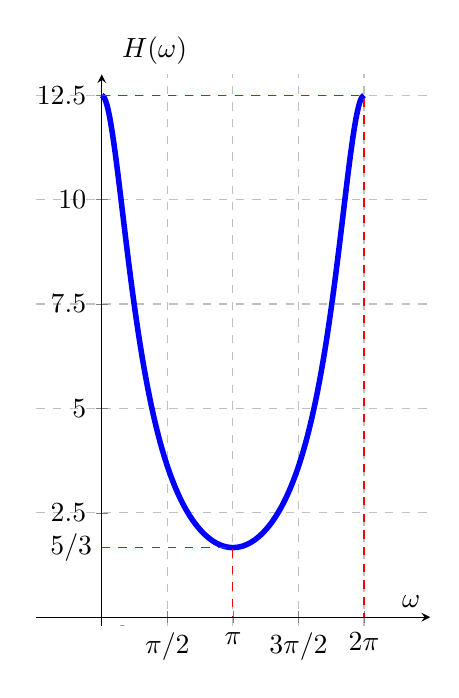
\begin{tikzpicture}
                    \begin{axis}[
                        axis lines = middle,
                        xlabel = {$\omega$},
                        ylabel = {$\abs{H(\omega)}$},
                        ylabel style={at={(rel axis cs:0.3, 1)}, anchor=south},
                        xmin = -0.2, xmax = 6.5,
                        ymin = -0.2, ymax = 13,
                        grid = major,
                        grid style = dashed,
                        scale only axis,
                        width = 5cm,
                        height = 7cm,
                        axis equal,
                        xtick = {0, 1.57, 3.14, 4.71, 6.28},
                        xticklabels = {$0$, $\pi/2$, $\pi$, $3\pi/2$, $2\pi$},
                        ytick = {0, 2.5, 5, 7.5, 10, 12.5},
                    ]
                    \addplot[domain=0:6.28, samples=100, smooth, line width=2pt, blue] {sqrt(17 + 8 * cos(deg(x))) / sqrt(1.5 + 0.2 * cos(deg(2 * x)) - 1.54 * cos(deg(x)))};
                    \addplot[dashed, red] coordinates {(0, 1.667) (3.14, 1.667) (3.14, 0)};
                    \addplot[dashed, red] coordinates {(0, 12.5) (6.28, 12.5) (6.28, 0)};
                    \node at (axis cs:0, 0) [anchor=north west] {O};
                    \node at (axis cs:0, 1.667) [anchor=east] {$5/3$};
                    \end{axis}
                \end{tikzpicture}
                \caption{习题 \theexercise~ 的系统幅频响应图}
                \label{fig:chap4-part2-exercise3}
            \end{figure}
            由图可知,该系统是低通滤波器。
        \item 只有 ROC 为 $\abs{z} > 0.5$ 时,包含单位圆,该系统是稳定的;其余情况下系统是不稳定的。
    \end{enumerate}
\end{solution}

\begin{note}
    在本题中,如果使用 $H(z) = (1 + 4z^{-1})W(z)$,则解答过程如下:
    \begin{align*}
        W(z) = \frac{1}{1 - 0.7z^{-1} + 0.1z^{-2}} = \frac{5/3}{1 - 0.5z^{-1}} - \frac{2/3}{1 - 0.2z^{-1}},
    \end{align*}
    则
    \begin{align*}
        w(n) = \begin{cases}
            -\frac{5}{3}(0.5)^nu(-n - 1) + \frac{2}{3}(0.2)^nu(-n - 1), & \abs{z} < 0.2, \\
            -\frac{5}{3}(0.5)^nu(-n - 1) - \frac{2}{3}(0.2)^nu(n), & 0.2 < \abs{z} < 0.5, \\
            \frac{5}{3}(0.5)^nu(n) - \frac{2}{3}(0.2)^nu(n), & \abs{z} > 0.5.
        \end{cases}
    \end{align*}
    由于 $H(z) = (1 + 4z^{-1})W(z) = W(z) + 4z^{-1}W(z)$,故 $h(n) = w(n) + 4w(n - 1)$。
    因此,其单位冲激响应为
    \begin{align*}
        h(n) = \begin{cases}
            -\frac{5}{3}(0.5)^nu(-n - 1) + \frac{2}{3}(0.2)^nu(-n - 1) \\
            \quad - \frac{20}{3}(0.5)^{n - 1}u(-n) + \frac{8}{3}(0.2)^{n - 1}u(-n), & \abs{z} < 0.2, \\
            -\frac{5}{3}(0.5)^nu(-n - 1) - \frac{2}{3}(0.2)^nu(n) \\
            \quad - \frac{20}{3}(0.5)^{n - 1}u(-n) - \frac{8}{3}(0.2)^{n - 1}u(n - 1), & 0.2 < \abs{z} < 0.5, \\
            \frac{5}{3}(0.5)^nu(n) - \frac{2}{3}(0.2)^nu(n) \\
            \quad + \frac{20}{3}(0.5)^{n - 1}u(n - 1) - \frac{8}{3}(0.2)^{n - 1}u(n - 1), & \abs{z} > 0.5.
        \end{cases}
    \end{align*}
    其中只有 ROC 为 $0.2 < \abs{z} < 0.5$ 时,包含单位圆,该系统是稳定的;其余情况下系统是不稳定的。
\end{note}

\subsection{数字滤波器的设计}

数字滤波器的设计分为两种,一种是\bd{有限脉冲响应}(FIR)滤波器的设计,
另一种是\bd{无限脉冲响应}(IIR)滤波器的设计。

\subsubsection{低通 FIR 滤波器的设计}

\begin{exercise}
    根据下列指标设计低通 FIR 滤波器,写出其单位冲激响应函数 $h(n)$。
    \begin{figure}[H]
        \centering
        \begin{tabular}{|c|c|}
            \hline
            通带边缘频率:$3.3\;\mathrm{kHz}$ & 过渡带宽度:$4.4\;\mathrm{kHz}$ \\
            \hline
            采样频率:$22\;\mathrm{kHz}$ & 阻带衰减:$43\;\mathrm{dB}$ \\
            \hline
        \end{tabular}
    \end{figure}
    供设计 FIR 滤波器时参考的各种窗函数性能如下图所示(若多种同时满足,则选序号最小的):
    \begin{figure}[H]
        \centering
        \begin{tabular}{|c|c|c|c|c|c|}
            \hline
            \textbf{序号} & \textbf{窗类型} & \textbf{窗函数} & \textbf{窗内项数} & \textbf{阻带衰减} & \textbf{通带边缘增益} \\
            \hline
            1 & 矩形 & $1$ & $0.91 f_s / \text{T.W.}$ & $21$ & $-0.9$ \\
            \hline
            2 & 汉宁 & $0.5 + 0.5\cos(2\pi n / (N-1))$ & $3.32 f_s / \text{T.W.}$ & $44$ & $-0.06$ \\
            \hline
            3 & 哈明 & $0.54 + 0.46\cos(2\pi n / (N-1))$ & $3.44 f_s / \text{T.W.}$ & $55$ & $-0.02$ \\
            \hline
            4 & 布莱克曼 & $0.42 + 0.5\cos(2\pi n / (N-1)) + 0.08\cos(4\pi n / (N-1))$ & $5.98 f_s / \text{T.W.}$ & $75$ & $-0.0014$ \\
            \hline
        \end{tabular}
    \end{figure}
\end{exercise}

\begin{solution}
    截止频率
    \begin{align*}
        f_c = 3.3 + \frac{1}{2} \times 4.4 = 5.5\;\mathrm{kHz},
    \end{align*}
    则
    \begin{align*}
        \omega_c = 2\pi \times \frac{f_c}{f_s} = 2\pi \times \frac{5.5}{22} = \frac{\pi}{2}.
    \end{align*}
    计算得
    \begin{align*}
        h(n) = \frac{\sin(\omega_c n)}{\pi n} = \frac{\sin(\pi n / 2)}{\pi n}.
    \end{align*}
    由阻带衰减为 $43\;\mathrm{dB}$ 知,应当选择汉宁窗。由于
    \begin{align*}
        N \ge 3.32 \times \frac{f_s}{T.W.} = 3.32 \times \frac{22}{4.4} = 16.6,
    \end{align*}
    故取 $N = 17$。则
    \begin{align*}
        w(n) = 0.5 + 0.5\cos\frac{2\pi n}{N - 1} = 0.5 + 0.5\cos\frac{\pi n}{8}.
    \end{align*}
    因此,低通 FIR 滤波器的冲激响应函数为
    \begin{align*}
        h'(n) = h(n) w(n) = \frac{\sin(\pi n / 2)}{\pi n} \left(0.5 + 0.5\cos\frac{\pi n}{8}\right) \quad (\abs{n} \le 8).
    \end{align*}
    将其右移 $(N-1)/2$ 个单位,即得
    \begin{align*}
        h''(n) = \frac{\sin(\pi (n - 8) / 2)}{\pi (n - 8)} \left(0.5 + 0.5\cos\frac{\pi (n - 8)}{8}\right) \quad (0 \le n \le 16).
    \end{align*}
\end{solution}



\subsubsection{带通 FIR 滤波器的设计}


\subsubsection{高通 FIR 滤波器的设计}

\begin{exercise}
    根据下列指标设计高通 FIR 滤波器,写出其单位冲激响应函数 $h(n)$。
    \begin{figure}[H]
        \centering
        \begin{tabular}{|c|c|}
            \hline
            通带边缘频率:$8.8\;\mathrm{kHz}$ & 过渡带宽度:$4.4\;\mathrm{kHz}$ \\
            \hline
            采样频率:$22\;\mathrm{kHz}$ & 阻带衰减:$35\;\mathrm{dB}$ \\
            \hline
        \end{tabular}
    \end{figure}
    供设计 FIR 滤波器时参考的各种窗函数性能如下图所示(若多种同时满足,则选序号最小的):
    \begin{figure}[H]
        \centering
        \begin{tabular}{|c|c|c|c|c|c|}
            \hline
            \textbf{序号} & \textbf{窗类型} & \textbf{窗函数} & \textbf{窗内项数} & \textbf{阻带衰减} & \textbf{通带边缘增益} \\
            \hline
            1 & 矩形 & $1$ & $0.91 f_s / \text{T.W.}$ & $21$ & $-0.9$ \\
            \hline
            2 & 汉宁 & $0.5 + 0.5\cos(2\pi n / (N-1))$ & $3.32 f_s / \text{T.W.}$ & $44$ & $-0.06$ \\
            \hline
            3 & 哈明 & $0.54 + 0.46\cos(2\pi n / (N-1))$ & $3.44 f_s / \text{T.W.}$ & $55$ & $-0.02$ \\
            \hline
            4 & 布莱克曼 & $0.42 + 0.5\cos(2\pi n / (N-1)) + 0.08\cos(4\pi n / (N-1))$ & $5.98 f_s / \text{T.W.}$ & $75$ & $-0.0014$ \\
            \hline
        \end{tabular}
    \end{figure}
\end{exercise}

\begin{solution}
    首先考虑其对应的低通 FIR 滤波器,截止频率
    \begin{align*}
        f_c = 11 - 8.8 + \frac{1}{2} \times 4.4 = 4.4\;\mathrm{kHz},
    \end{align*}
    则
    \begin{align*}
        \omega_c = 2\pi \times \frac{f_c}{f_s} = 2\pi \times \frac{4.4}{22} = \frac{2\pi}{5}.
    \end{align*}
    计算得
    \begin{align*}
        h(n) = \frac{\sin(\omega_c n)}{\pi n} = \frac{\sin(2\pi n / 5)}{\pi n}.
    \end{align*}
    由阻带衰减为 $35\;\mathrm{dB}$ 知,应当选择汉宁窗。由于
    \begin{align*}
        N \ge 3.32 \times \frac{f_s}{T.W.} = 3.32 \times \frac{22}{4.4} = 16.6,
    \end{align*}
    故取 $N = 17$。则
    \begin{align*}
        w(n) = 0.5 + 0.5\cos\frac{2\pi n}{N - 1} = 0.5 + 0.5\cos\frac{\pi n}{8}.
    \end{align*}
    因此,高通 FIR 滤波器的冲激响应函数为
    \begin{align*}
        h'(n) = h(n) w(n) \cos\pi n = \frac{\sin(2\pi n / 5)}{\pi n} \left(0.5 + 0.5\cos\frac{\pi n}{8}\right) \cos\pi n \quad (\abs{n} \le 8).
    \end{align*}
    将其右移 $(N-1)/2$ 个单位,即得
    \begin{align*}
        h''(n) = \frac{\sin(2\pi (n - 8) / 5)}{\pi (n - 8)} \left(0.5 + 0.5\cos\frac{\pi (n - 8)}{8}\right) \cos\pi (n - 8) \quad (0 \le n \le 16).
    \end{align*}
\end{solution}

